\chapter{Sistemas dinâmicos de medida}

\begin{definition}
Um \emph{sistema dinâmico de medida} (ou \emph{sistema que preserva medida}) é uma dupla $\bm{\Sist}=(\bm X,f)$ em que $\bm X$ é um espaço de medida, $(X,f)$ é um sistema dinâmico e $f$ é uma ação que preserva medida em $\bm X$.
\end{definition}

Como estudaremos somente o caso \textbf{discreto}, a função $f$ é no caso um morfismo de medida, uma função que preserva a medida do espaço. Ainda, estudaremos somente \textbf{espaços de probabilidade}. Introduzimos agora noções de morfismo de sistemas dinâmicos de probabilidade. Em geral, quando tratamos da teoria da medida, podemos considerar funções que são iguais a menos de um conjunto de medida nula.

\section{Conjugação que preserva medida}

\begin{definition}
Sejam $\bm{\Sist_1} = (\bm{X_1},f_1)$ e $\bm{\Sist_2} = (\bm{X_2},f_2)$ sistemas que preservam medida. Uma \emph{semiconjugação de medida} de $\bm{\Sist_1}$ para $\bm{\Sist_2}$ é uma semiconjugação $\phi: C_1 \to C_2$ que preserva medida, definida em conjuntos mensuráveis $C_1 \in \mens_1$ e $C_2 \in \mens_2$ que satisfazem ${f_1}(C_1) \subseteq C_1$, ${f_2}(C_2) \subseteq C_2$ e $\med_1(C_1) = \med_2(C_2) = 1$. Nesse caso, o sistema $\bm{\Sist_2}$ é um \emph{fator} do sistema $\bm{\Sist_1}$. Uma \emph{conjugação de medida} de $\bm{\Sist_1}$ para $\bm{\Sist_2}$ é uma semiconjugação de medida que é uma conjugação.

\begin{figure}
\centering
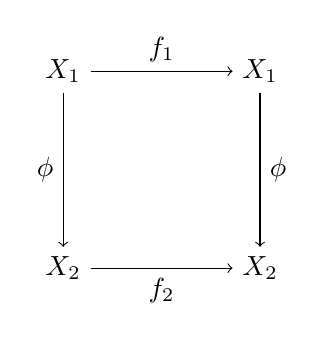
\begin{tikzpicture}[node distance=2.5cm, auto]
	\node (X) {$X_1$};
	\node (XX) [right of=X] {$X_1$};
	\node (Y) [below of=X] {$X_2$};
	\node (YY) [right of=Y] {$X_2$};
	\draw[->] (X) to node {$f_1$} (XX);
	\draw[->] (X) to node [swap] {$\phi$} (Y);
	\draw[->] (Y) to node [swap] {$f_2$} (YY);
	\draw[->] (XX) to node {$\phi$} (YY);
\end{tikzpicture}
\end{figure}
\end{definition}

%Isso é o mesmo que dizer que $\phi: X_1 \to X_2$ é uma quase função sobrejetiva que preserva medida com domínio e contradomínio positivamente invariantes.

Como comentado anteriormente, podemos considerar $\phi$ como definida de $X_1$ para $X_2$ sem problemas, pois só não está definida em um conjunto de medida nula.

\section{Recorrência}

%\begin{theorem}\label{teo:recorrencia.poincare}
%Seja $(\bm X,f)$ um sistema dinâmico que preserva medida. Para todo conjunto mensurável $E \in \mens$ com $\med(E)>0$, existe um conjunto mensurável $F \subseteq E$, com $\med(F)=\med(E)$, tal que se $x \in F$, então existe uma sequência de inteiros $0<n_0<n_1< n_2 < \ldots$ satisfazendo que, para todo $i \in \N$
%	\begin{equation*}
%	f^{n_i}(x) \in E.
%	\end{equation*}
%\end{theorem}
\begin{theorem}[Recorrência]
\label{teo:sd.poincare}
Sejam $(\bm X,f)$ um sistema dinâmico de medida finita e $M \in \mens$ um conjunto mensurável. Então quase todo ponto de $M$ retorna infinitamente a $M$:
%	\begin{equation*}
%	\med\left( \set{x \in M}{\card{\Orb^+(x) \cap M} = \card{\N}} \right) = \med(M).
%	\end{equation*}
	\begin{equation*}
	\set{x \in M}{\card{\Orb^+(x) \cap M} = \card{\N}} \qeq M.
	\end{equation*}
\end{theorem}
\begin{proof}
Se $M \qeq \emptyset$, a proposição é evidente. Suponhamos $M \not\qeq \emptyset$.
Notemos que
	\begin{equation*}
	\set{x \in M}{\card{\Orb^+(x) \cap M} = \card{\N}} = M \cap \limsup_{t \in \I^+} f^{-t}(M).
	\end{equation*}
Esse é o conjunto dos pontos de $M$ que retornam infinitamente para $M$. Queremos provar que esse conjunto tem a mesma medida de $M$. Consideremos os conjuntos
	\begin{equation*}
	M_N := \bigcup_{n=N}^\infty f^{-n}(M).
	\end{equation*}
%os conjuntos dos pontos cujas órbitas passam por $M$ após $N$ iterações da dinâmica.
Temos que $f^{-1}(M_N)=M_{N+1}$, e, como $f$ preserva $\med$, segue que $\med(M_N)=\med(M_{N+1})$. Isso implica que $\med(M_0)=\med(M_N)$ para todo $N \in \N$. Observe que $M_0 \supset M_1 \supset M_2 \ldots$, então segue, pelo lema \ref{lema:medida.inter.decre}, que
	\begin{equation*}
	\med\left( \bigcap_{N=0}^\infty M_N \right) = \lim_{N \to \infty} \med(M_N) = \med(M_0).
	\end{equation*}
Notando que $\bigcap_{N=0}^\infty M_N = \limsup_{t \in \I^+} f^{-t}(M)$, consequentemente segue que
	\begin{equation*}
	\med(F)= \med\left(M \cap \limsup_{t \in \I^+} f^{-t}(M) \right) =\med(M\cap M_0)=\med(M).
	\end{equation*}
A segunda igualdade segue de $\bigcap_{N=0}^\infty M_N = M_0$ quase sempre, e a terceira vem de $M \subseteq M_0$.
\end{proof}

Como mencionado antes, a hipótese de que o sistema tem medida finita é fundamental para usar o lema \ref{lema:medida.inter.decre}.

\begin{proposition}
Seja $\bm{\Sist}=(\bm X,f)$ um sistema dinâmico topológico, $\bm X$ com base enumerável. O conjunto $\Rec(f)$ dos pontos recorrentes é mensurável (com respeito à $\sigma$-álgebra gerada pela topologia).
\end{proposition}
\begin{proof}
Basta notar que a igualdade da proposição~\ref{prop:recorr} é uma interseção enumerável de conjuntos mensuráveis.
\end{proof}


\begin{theorem}[Recorrência Topológica]
\label{teo:sd.top.poincare}
Seja $\bm{\Sist}=(\bm X,f)$ um sistema dinâmico topológico de medida. Se a topologia de $\bm X$ tem base enumerável, quase todo ponto é recorrente:
	\begin{equation*}
	\Rec(f) \qeq X.
	\end{equation*}
\end{theorem}
\begin{proof}
Seja $(A_i)_{i \in \N}$ uma base enumerável da topologia de $\bm X$. Pelo teorema~\ref{teo:sd.poincare}, existe $\tilde A_i \subseteq A_i$ tal que $\med(\tilde A_i) = 0$, o conjunto dos $x \in A_i$ que retornam para $A_i$ finitas vezes. Defina
	\begin{equation*}
	\tilde M := M \setminus \bigcup_{i \in \N} \tilde A_i.
	\end{equation*}
Temos que $\med(\tilde M) = 1$, pois $\med(\bigcup_{i \in \N} \tilde A_i) \leq \sum_{i \in \N} \med(\tilde A_i) = 0$.

Queremos mostrar que $\tilde M \subseteq \Rec(f)$. Seja $x \in \tilde M$. Dado vizinhança $A$ de $x$, queremos encontrar $n \in \N$ tal que $f^n(x) \in A$. Como $(A_i)_{i \in \N}$ é base, existe $i \in \N$ tal que $x \in A_i \subseteq A$. Como $x \in \tilde M$, então $x \notin \tilde A_i$, portanto existe $n \in \N$ tal que $f^n(x) \in A_i$, logo $f^n(x) \in A$.
\end{proof}





\section{Teoremas ergódicos}

\subsection{Tempo médio de visita}

Começamos definindo o conceito de tempo médio de visita para motivar os enunciados dos teoremas ergódicos.

\begin{definition}
Sejam $(\bm X,f)$ um sistema dinâmico de medida, $M \subseteq X$ um conjunto mensurável de medida não nula. Para todo $x \in X$, o \emph{tempo médio de visita} de $x$ em $M$ é
	\begin{equation*}
	\tau_M(x) := \lim_{n \to \infty} \frac{1}{n} \#\left(\set{t \in [n]}{f^t(x) \in M}\right).
	\end{equation*}

No caso de um sistema contínuo, definimos
	\begin{equation*}
	\tau_M(x) := \lim_{n \to \infty} \frac{1}{n} \vol^1\left(\set{t \in \intfa{0}{n}}{f^t(x) \in M}\right),
	\end{equation*}
em que $\vol^1$ é a medida de volume unidimensional em $\R$.
\end{definition}

Esses limites não necessariamente existem para todos pontos. Podemos reescrever a equação de $\tau_M(x)$ como
	\begin{equation*}
	\widehat{f}(\idc_M)(x) = \lim_{n \to \infty} \frac{1}{n} \sum_{t \in [n]} \idc_M(f^t(x)) = \lim_{n \to \infty} \frac{1}{n} \sum_{t \in [n]} ({f^t}\emp \idc_M) (x).
	\end{equation*}
 Ainda, podemos escrever
	\begin{equation*}
	\widehat{f}(\idc_M) = \lim_{n \to \infty} \frac{1}{n} \sum_{t \in [n]} \idc_{f^{-t}(M)} = \lim_{n \to \infty} \frac{1}{n} \sum_{t \in [n]} \idc_{f^{-t}(M)}.
	\end{equation*}

Podemos considerar casos mais gerais de funções $\phi \in \Men(X,\R)$ e perguntar se o limite
	\begin{equation*}
	\widehat{f}(\phi) = \lim_{n \to \infty} \frac{1}{n} \sum_{t \in [n]} \phi \circ f^t = \lim_{n \to \infty} \frac{1}{n} \sum_{t \in [n]} {f^t}\emp \phi.
	\end{equation*}

Os teoremas ergódicos vai tratar sobre esses limites.

\subsection{Média temporal e média espacial}

\begin{definition}
Sejam $(\bm X,f)$ um sistema dinâmico de medida e $\phi \in L^1(X,\R)$.
	\begin{enumerate}
	\item A \emph{média temporal} de $\phi$ em $(\bm X,f)$ é a quase-função
		\begin{equation*}
		\widehat{\phi} := \lim_{n \to \infty} \frac{1}{n} \sum_{t \in [n]} \phi \circ f^t = \lim_{n \to \infty} \frac{1}{n} \sum_{t \in [n]} {f^t}\emp(\phi);
		\end{equation*}

	\item Se $\med$ é finita e não nula, a \emph{média espacial} de $\phi$ em $(\bm X,f)$ é
		\begin{equation*}
		\overline{\phi} := \frac{1}{\med(X)} \int \phi.
		\end{equation*}
	\end{enumerate}
\end{definition}

Podemos pensar na média temporal como um operador
	\begin{equation*}
	\widehat{\var} := \lim_{n \to \infty} \frac{1}{n} \sum_{t \in [n]} {f^t}\emp.
	\end{equation*}
Mais explicitamente,
	\begin{align*}
	\func{\widehat{\var}}{L^1(X,\R)}{L^1(X,\R)}{\phi}{\lim_{n \to \infty} \frac{1}{n} \sum_{t \in [n]} {f^t}\emp(\phi)}.
	\end{align*}
Esse operador é linear e, como veremos, preserva a norma $1$.

%Além disso, podemos pensar na média espacial como o operador

\subsection{Teorema ergódico da média}

\begin{theorem}[Ergódico da Média\footnote{Este teorema é conhecido como Teorema Ergódico de Von Neumann, em homenagem ao matemático húngaro \textit{John von Neumann} (28/12/1903 -- 08/02/1957).}]
Seja $(\bm X,f)$ um sistema dinâmico de medida e $\proj\colon \Intg^2(X,\R) \to (f\emp - \Id)\inv(0)$ a projeção no subespaço
	\begin{equation*}
	(f\emp - \Id)\inv(0) = \set{\phi \in \Intg^2(X,\R)}{f\emp \phi = \phi \circ f = \phi}.
	\end{equation*}
Para toda função $\phi \in \Intg^2(X,\R)$,
	\begin{equation*}
	\lim_{n \to \infty} \frac{1}{n} \sum_{i \in [n]} {f^i}\emp \phi \conv \proj \phi.
	\end{equation*}
\end{theorem}


\subsection{Teorema ergódico pontual}

\begin{theorem}[Ergódico Pontual\footnote{Este teorema é conhecido como Teorema Ergódico de Birkhoff, em homenagem ao matemático estadunidense \textit{George David Birkhoff} (21/03/1884 -- 12/11/1944).}]
Seja $(\bm X,f)$ um sistema dinâmico de medida ($\sigma$-finita). Para toda função $\phi \in L^1(X,\R)$, existe $\widehat{\phi} \in \Intg^1(X,\R)$ $f$-invariante tal que, para quase todo $x \in X$,
	\begin{equation*}
	\widehat{\phi}(x) = \lim_{n \to \infty} \frac{1}{n} \sum_{i \in [n]} \phi \circ f^i(x).
	\end{equation*}
Se a medida é finita, então
	\begin{equation*}
	\int \widehat{\phi} = \int \phi.
	\end{equation*}
\end{theorem}

\begin{proposition}
Seja $(\bm X,f)$ um sistema dinâmico de medida (probabilidade). São equivalentes
	\begin{enumerate}
	\item Para toda $\phi \in \Intg^1(X,\R)$, $\widehat{\phi}$ é quase constante;

	\item Para toda $\phi \in \Intg^1(X,\R)$, $\widehat{\phi} = \int \phi$;

	\item Para toda $\phi \in \Intg^1(X,\R)$, se $\phi$ é quase $f$-invariante, então é quase constante.

	\item Todo conjunto mensurável invariante ($f\inv(M) = M$) é quase vazio ou quase total ($\med(M) = 0$ ou $\med(M) = 1$);

	\item Todo conjunto mensurável negativamente invariante ($f\inv(M) \subseteq M$) é quase vazio ou quase total;

	\item Todo conjunto mensurável $M \subseteq X$ tal que $M \subseteq f\inv(M)$ (positivamente invariante?) é quase vazio ou quase total.
	\end{enumerate}
\end{proposition}
% DEMONSTRAÇÃO: Usar a função característica de um conjunto mensurável.

Essas proposições são a definição de um sistema dinâmico ergódico, como veremos na seção seguinte.

\section{Ergodicidade}

Nesta seção, introduziremos o conceito de ergodicidade. A definição de transformação em sistemas ergódicos virá seguida de uma proposição que mostra várias equivalências de propriedades que caracterizam a ergodicidade. Essas equivalências são importantes não só como resultados teóricos interessantes e importantes ferramentas da teoria, mas também como embasamento intuitivo da ideia de ergodicidade. Relembramos que um conjunto é quase vazio quando tem medida $0$ e quase total quando seu complementar tem medida $0$.

\begin{definition}
Um \emph{sistema dinâmico ergódico} é um sistema dinâmico de medida $\bm\Sist=(\bm X,f)$ tal que todo conjunto mensurável invariante de $\bm\Sist$ é quase vazio ou quase total: para todo $M \in \mens$ tal que $f\inv(M) = M$, $M \qeq \emptyset$ ou $M \qeq X$. A dinâmica $f$ é uma \emph{dinâmica ergódica}.
\end{definition}

\begin{proposition}
Seja $\bm\Sist=(\bm X,f)$ um sistema dinâmico de medida. São equivalentes
	\begin{enumerate}
	\item $f$ é ergódica;
	\item Todo conjunto quase invariante de $\bm\Sist$ é quase vazio ou quase total (para todo $M \in \mens$ tal que $f^{-1}(M) \qeq M$, $M \qeq \emptyset$ ou $M \qeq X$);
	\item A semiórbita positiva de quase todo ponto passa por qualquer conjunto de medida positiva: para todo $M \in \mens$ tal que $M \not\qeq \emptyset$,
		\begin{equation*}
		\bigcup_{n \in \I^+} f^{-n}(M) = \set{x \in X}{\Orb^+(x) \cap M \neq \emptyset} \qeq X;
		\end{equation*}
	\item Se a semiórbita positiva de quase nenhum ponto de um conjunto mensurável passa por um outro conjunto mensurável, algum dos conjuntos é quase vazio: para todos $N,M \in \mens$ tais que
	\begin{equation*}
	N \cap \bigcup_{n \in \I^+}f^{-n}(M) \qeq \emptyset,
	\end{equation*}
$N \qeq \emptyset$ ou $M \qeq \emptyset$.
%	Para todos $M,N \in \mens$ tais que $M \not\qeq \emptyset$ e $N \not\qeq \emptyset$, existe $n \in \I^+$ tal que
%		\begin{equation*}
%		N \cap f^{-n}(M) \not\qeq \emptyset;
%		\end{equation*}
	\end{enumerate}
\end{proposition}
\begin{proof}
(1) $\Rightarrow$ (2) Pela proposição \ref{prop:quase.inv}, existe um conjunto invariante $N \in \mens$ tal que $M \qeq N$. Pela ergodicidade, segue que $N \qeq \emptyset$ ou $N \qeq X$, portanto segue que $M \qeq \emptyset$ ou $M \qeq X$.

(2) $\Rightarrow$ (3) Seja $M \in \mens$ com $\med(M)>0$ e definamos
	\begin{equation*}
	N := \bigcup_{n \in \I^+} f^{-n}(M).
	\end{equation*}
Segue que $f\inv(N) \subseteq N$. Isso implica que $f\inv(N) \cup N= N$ e que $f\inv(N) \cap N = f\inv(N)$. Portanto, como $\med(f\inv(N))=\med(N)$, pois $f$ preserva medida, segue que
	\begin{align*}
	\med(N \difsim f\inv(N)) &= \med(f\inv(N) \cup N) - \med(f\inv(N) \cap N) \\
		&= \med(N) - \med(f\inv(N)) = 0.
	\end{align*}
Assim, temos que $f\inv(N) \qeq N$, e de (2) segue que $N \qeq \emptyset$ ou $N \qeq X$. Mas $N \not\qeq \emptyset$, pois $f\inv(M) \subseteq N$ e $\med(f\inv(M))=\med(M) > 0$, logo temos que $N \qeq X$.

(3) $\Rightarrow$ (4) Vamos provar a recíproca. Sejam $M,N \in \mens$ tais que $M \not\qeq \emptyset$ e $N \not\qeq \emptyset$. Por (3), sabemos que
	\begin{equation*}
	\med\left(\bigcup_{n \in \I^+} f^{-n}(M)\right)=1,
	\end{equation*}
e disso segue que
	\begin{equation*}
	0 < \med(N) = \med\left(\bigcup_{n \in \I^+} N \cap f^{-n}(M)\right) \leq \sum_{n \in \I^+} \med(N \cap f^{-n}(M)).
	\end{equation*}
Logo, existe $n \in \I^+$ tal que $\med(N \cap f^{-n}(M))>0$.

(4) $\Rightarrow$ (1) Seja $M \in \mens$ tal que $f\inv(M)=M$. Então segue que $f^{-n}(M)=M$ para todo $n \in \I^+$, logo
	\begin{equation*}
	0=\med(M \cap M^\complement)=\med(f^{-n}(M) \cap M^\complement)
	\end{equation*}
para todo $n \in \I^+$, o que implica por (4) que $M \qeq \emptyset$ ou $M^\complement \qeq \emptyset$, logo $M \qeq \emptyset$ ou $M \qeq X$, e a ergodicidade está provada.
\end{proof}

\begin{proposition}
	\begin{enumerate}
	\item A rotação $R_\alpha$ no círculo é ergódica se, e somente se, $\alpha$ é irracional.
	\item O shift de Bernoulli é ergódico.
	\item A expansão no círculo é ergódica.
	\end{enumerate}
\end{proposition}
\begin{proof}
\begin{enumerate}
	\item Se $\alpha \in \Q$, escrevemos $\alpha=\frac{p}{q}$ fração reduzida. Então, tomando um conjunto mensurável $A \subseteq \T$ tal que $)<\med(A)<\frac{1}{q}$, segue que o conjunto
	\begin{equation*}
	M := A \cup R_{\alpha}(A) \cup R^2_{\alpha}(A) \cap \cdots \cup R^{q-1}_{\alpha}(A)
	\end{equation*}
é invariante sob $R_{\alpha}$, pois $R_{\alpha}^q=id_{\T}$. No entanto, $0<\med(M)< 1$, o que mostra que $\R_\alpha$ não é ergódica.

	Se $\alpha \notin \Q$, então a rotação é densa em $\T$. Sendo assim, seja $M \subseteq \T$ invariante sob $R_\alpha$. Podemos escolher, para todo $\varepsilon$ uma função $f$  contínua no toro tal que $\Vert f-\idc_M \Vert_1 < \varepsilon$ e da invariância de $M$ segue que $\Vert f\circ R^n_\alpha-f\Vert_1<2\varepsilon$. Da continuidade de $f$, segue que, para todo $t \in \R$, $\Vert f\circ R_t-f\Vert_1\leq2\varepsilon$. Agora, como a medida é invariante por rotação, usando o teorema de Fubini e a desigualdade triangular para integrais temos que
	\begin{align*}
	\left\Vert f-\int f(t) dt\right\Vert_1 &= \int\left|\int (f(x)-f(x+t))dt \right|dx \\
	&\leq \int \int |f(x)-f(x+t)|dxdt \\
	&\leq 2\varepsilon.
	\end{align*}
Mas então
	\begin{equation*}
	\Vert \idc_M-\med(M) \Vert_1 \leq \Vert\idc_m-f\Vert_1+\left\Vert f-\int f(t) dt\right\Vert_1+\left\Vert \int f(t) dt-\med(M)\right\Vert_1<4\varepsilon.
	\end{equation*}
Concluímos, portanto, que $\idc_M$ é constante, pois isso vale para qualquer $\varepsilon$. Mas então $\med(M)$ é $0$ ou $1$, logo $R_\alpha$ é ergódica.

	\item Seja $N \in \mens$ invariante. Para qualquer $\varepsilon>0$, existe uma união finita de cilindros $M$ tais que $\med(M \difsim N)<\varepsilon$, o que implica $|\med(M)-\med(N)|<\varepsilon$. O conjunto $M$ pode ser escrito como
	\begin{equation*}
	M = \{x \in X: x_{-m}\cdots x_m \in F\}
	\end{equation*}
para algum $m$ e $F \subseteq \{0,1,\cdots,n\}^{\{-m,\cdots,m\}}$. Assim, para todo $k>2m$, temos que
	\begin{equation*}
	\sigma^{-k}(M)=\{x \in X: x_{k-m}\cdots x_{k+m} \in F\}.
	\end{equation*}
Como esse dois conjuntos são independentes, segue que
	\begin{equation*}
	\med\left(\sigma^{-k}(M) \setminus M\right) = \med\left(\sigma^{-k}(M) \cap M^ \complement\right)=\med\left(\sigma^{-k}(M)\right)\med\left(M^\complement\right)=\med(M)\med\left(M^\complement\right).
	\end{equation*}
	Como $N$ é invariante, temos que $\med(N \difsim \sigma^{-1}(M))$, e então
	\begin{equation*}
	\med(\sigma^{-k}(M) \difsim N) =\med(\sigma^{-k}(M) \difsim \sigma^{-k}(N))=\med(M \difsim N)<\varepsilon
	\end{equation*}
logo $\med(\sigma^{-k}(M) \difsim M)<2\varepsilon$ e
	\begin{equation*}
	\med(\sigma^{-k}(M) \setminus M)+\med(M \setminus \sigma^{-k}(M)) = \med(\sigma^{-k}(M) \difsim M) < 2\varepsilon.
	\end{equation*}
Finalmente, obtemos que
	\begin{align*}
	\med(N)\med\left(N^\complement\right)&<(\med(M)+\varepsilon)(\med(M^\complement)+\varepsilon) \\
	&=\med(M)\med(M^\complement)+\varepsilon\mu(M)+\varepsilon\mu(M^\complement)+\varepsilon^2 \\
	&<2\varepsilon+\varepsilon+\varepsilon^2.
	\end{align*}
Como isso vale para qualquer $\varepsilon$, segue que $\med(N)\med\left(N^\complement\right)=0$; ou seja, que $\med(N)$ é $0$ ou $1$, logo o sistema é ergódico.

	\item Como os sistemas de Bernoulli $\Sigma$ e a expansão $E_2$ são isomorfos por medida, segue que a expansão é ergódica.
\end{enumerate}
\end{proof}

\section{Sistemas misturadores}

Nesta seção consideraremos duas noções de um sistema misturador: a de \emph{misturador} e de \emph{fracamente misturador}. Um sistema misturador também é conhecido como fortemente misturador para distinguí-lo dos fracamente misturadores. Existem, de fato, outras noções de misturador, que generalizam a ideia de misturador, como \emph{misturador de ordem $k$} (cf. \cite{ein}), mas aqui consideraremos apenas essas duas. Antes de introduzir a definição, vale ressaltar uma outra definição equivalente de sistema ergódico, enunciada abaixo, cuja demonstração pode ser achada em \cite{ein}. Essa classificação é uma consequência do teorema da média ergódica.

\begin{proposition}
	Um sistema $(X,\mens,\med,T)$ é ergódico se, e somente se, para todos $M,N \in \mens$,
	\begin{equation*}
	\frac{1}{n} \sum_{i=0}^{n-1} \med(M \cap T^{-i}(N)) \conv \med(M)\med(N)
	\end{equation*}
quando $n \conv \infty$.
\end{proposition}

	A definição a seguir, de um sistema misturador, destaca a seguinte ideia. Em alguns sistema, se tomamos dois subconjuntos mensuráveis quaisquer dos espaços, notamos que sempre ocorre que um deles é independente da $n$-ésima imagem inversa do outro quando $n$ é grande. O sentido de independência empregado é que, em espaços de probabilidade, eventos são pensados como conjuntos mensuráveis e dois eventos $E,F$ são independentes quando $\med(E \cap F)=\med(E)\med(F)$; ou seja, a probabilidade dos dois ocorrerem é o produto das probabilidades de cada um deles ocorrer separadamente. Pensando em conjuntos, e agora considerando uma ideia geométrica que motiva o nome \emph{misturador}, essa ideia é equivalente a pensar que os conjuntos, quando iterados, estão muito bem separados no sistema, misturados, de modo que se fixamos um deles, o primeiro, a medida das imagens inversas do segundo que estão nesses primeiro conjunto dividida pela medida desse primeiro é igual à medida do segundo; ou seja, a quantidade do segundo que está no primeiro é proporcionalmente igual à quantidade desse segundo no espaço todo. A definição a seguir formaliza o que foi aqui explicado.

\begin{definition}
	Um sistema \emph{misturador} é um sistema $(X,\mens,\med,T)$ que preserva medida tal que, para todos $M,N \in \mens$,
	\begin{equation*}
	\med(M \cap T^{-n} N) \conv \med(M)\med(N)
	\end{equation*}
quando $n \conv \infty$
\end{definition}

\begin{proposition}
	A rotação $R_\alpha$ no círculo não é misturadora.
\end{proposition}
\begin{proof}
	Tomando uma sequência $n_i \to \infty$ tal que $n_i\alpha \mod 1 \conv 0$. No caso de $\alpha$ irracional isso é possível pois a rotação é densa, e no caso de racional, basta tomar uma sequência constante igual a zero. Tomando os conjuntos $M=N=[0,\frac{1}{2}]$, segue que, quando $i \conv \infty$,
	\begin{equation*}
	\med(M \cap R_\alpha^{-n_i}(N))=\med(M \cap R_{-n_i\alpha}(M)) \conv \med(M)=\frac{1}{2}\neq \left(\frac{1}{2}\right)^2=\med(M)\med(N).
	\end{equation*}
\end{proof}

	Embora o conceito de sistema misturador como definido acima é mais natural, a noção levemente modificada abaixo é, muitas vezes, mais útil e simples de se aplicar. Esse é o conceito de fracamente misturador.

\begin{definition}
	Um sistema \emph{fracamante misturador} é um sistema $(X,\mens,\med,T)$ tal que, para todos $M,N \in \mens$,
	\begin{equation*}
	\frac{1}{n} \sum_{i=0}^{n-1} \left|\med(M \cap T^{-i}(N)) - \med(M)\med(N)\right| \conv 0
	\end{equation*}
quando $n \conv \infty$
\end{definition}

	É interessante comentar algo sobre os diferentes tipos de convergência aqui considerados. Além da convegência tradicional, $a_n \conv a$, existem outras noções de convergência de uma sequência. Uma delas é convergência de Cesàro, que considera a convergência da sequência $\frac{1}{n} \sum_{i=0}^{n-1} a_n$ das $n$-ésimas médias da sequência original. Pelas definições e proposições anteriores, considrando a sequência $a_i\coloneqq\med(M \cap T^{-i}(N)) - \med(M)\med(N)$, temos que um sistema é \emph{ergódico} se, e somente se, $a_n$ converge a $0$ pela convergência de Cesàro, é \emph{misturador} se, e somente se, $a_n$ converge a $0$ no sentido tradicional, e é \emph{fracamente misturador} se $|a_n|$ converge a $0$ pela convergência de Cesàro. Assim, como, para qualquer sequência $a_n$ que converge a $0$, vale que $|a_n|$ converge a $0$ por Cesàro e, então, $a_n$ converge a $0$ por Cesàro, segue a proposição abaixo.

\begin{proposition}
	Seja $(X,\mens,\med,T)$ um sistema que preserva medida. Então
	\begin{enumerate}
	\item Se o sistema é misturador, é fracamente misturador.
	\item Se o sistema é fracamente misturador, é ergódico.
	\end{enumerate}
\end{proposition}
\begin{proof}
	Basta considerar a sequência $a_i\coloneqq\med(M \cap T^{-i}(N)) - \med(M)\med(N)$ e os comentários do parágrafo anterior.
\end{proof}

\begin{definition}
	A \emph{densidade} de um conjunto $C \subseteq \N$ é o número
	\begin{equation*}
	d(C) \coloneqq \lim_{n \to \infty} \frac{1}{n} \left|\{k \in C: 0 \leq k < n\}\right| = \frac{1}{n} \left|(C \cap [0,n)\right|
	\end{equation*}
quando o limite existir.
\end{definition}

	Antes de demonstrar um teorema importante a seguir com várias equivalências envolvendo a propriedade de ergodicidade e mistura fraca, demonstraremos um lema sobre convergência de sequências.

\begin{lemma}
	Seja $(a_n)_{n \in \N}$ uma sequência limitada de números reais positivos. São equivalentes as seguintes noções de convergência.
	\begin{enumerate}
	\item $\lim_{n \to \infty} \frac{1}{n} \displaystyle\sum_{i=0}^{n-1} a_i =0$.
	\item Existe um conjunto $C \subseteq \N$ com densidade zero tal que $a_n \conv 0$ para $n \conv \infty$, $n \notin C$.
	\item $\lim_{n \to \infty} \frac{1}{n} \displaystyle\sum_{i=0}^{n-1} a_i^2 =0$.
	\end{enumerate}
\end{lemma}
\begin{proof}
Vamos mostrar que (1) implica (2). Definamos $C_k \coloneqq \{j \in \N:a_j>\frac{1}{k}\}$. Então temos que
	\begin{equation}
	C_1 \subseteq C_2 \subseteq C_3 \subseteq \cdots,
	\end{equation}
pois, se $x \in C_k$, então $x >\frac{1}{k}>\frac{1}{k+1}$, logo $x \in C_{k+1}$. Então temos que, para todo $k \geq 1$,
	\begin{equation*}
	\frac{1}{k} |C_k \cap [0,n)| = \sum_{i \in C_k \cap [0,n)} \frac{1}{k} < \sum_{i \in C_k \cap [0,n)} a_i \leq \sum_{i=0}^n a_i
	\end{equation*}
e então segue que
	\begin{equation*}
	\frac{1}{n}  |C_k \cap [0,n)| \leq k\frac{1}{n}\sum_{i=0}^n a_i \conv 0
	\end{equation*}
quando $n \conv \infty$. Logo, para todo $k \geq 1$, $C_k$ tem densidade $0$. Como cada $C_k$ tem densidade $0$, podemos escolher inteiros $0<l_1<l_2<\cdots$ tais que, para todo $k \geq 1$ e para todo $n \geq l_k$,
	\begin{equation}
	\frac{1}{n}  |C_k \cap [0,n)| \leq \frac{1}{k}.
	\end{equation}
Basta escolher $l_1$ e tomar um $l_2$ suficientemente grande e assim por diante. Definimos então o conjunto
	\begin{equation}
	C \coloneqq \bigcup_{k \in \N} \left(C_k \cap [l_k,l_{k+1})\right).
	\end{equation}
Vamos mostrar que $a_i$ converge a $0$ para $n \notin C$ e que $C$ tem densidade $0$. Primeiro, notamos que $C_k \cap [l_k,\infty) \subseteq C$, pois, se $x \in C_k$, então está em todo $C_p$ para $p \geq k$, e, então, se estiver em $[l_p,l_{p+1})$, estará em $C_p \cap [l_p,l_{p+1})$, logo em $C$. Assim, para todo $n \geq l_k$, então se $n \notin C$, temos $n \notin C_k$ e, portanto, $a_n \leq \frac{1}{k}$, logo $a_n \conv 0$. Agora, para mostrar que $C$ tem densidade zero, notemos que, para todo $n \in [l+k,l_{k+1})$ temos que $C \cap [0,n) \subseteq C_k \cap [0,n)$, pois se $x \in C \cap [0,n)$, está em algum $[l_p,l_{p+1})$ e, por consequência, em $C_k \cap [0,n)$, já que todo $C_p$ está contido no $C_k$ para $p \leq k$. Isso implica que
	\begin{equation}
	\frac{1}{n} |C \cap [0,n)| \leq \frac{1}{n}  |C_k \cap [0,n)| \leq \frac{1}{k}
	\end{equation}
e, portanto, $C$ tem densidade zero.

Agora, vamos mostrar que (2) implica (1). Como a sequêcia é limitada, seja $L>0$ tal que $a_n \leq L$ para todo $n \geq 1$. Como $a_n$ converge para zero fora de $C$ e o conjunto $C$ tem densidade zero, podemos escolher, para cada $k \geq 1$, $n_k \in \N$ tal que, para todo $n \notin C$, $n \geq n_k$, temos que $a_n < \frac{1}{k}$ e, para todo $n \geq n_k$, $\frac{1}{n}|C \cap [0,n)| \leq \frac{1}{k}$. Sendo assim, para todo $n \geq kn_k$, temos que
	\begin{align*}
	\frac{1}{n} \sum_{i=0}^{n-1} a_i &= \frac{1}{n} \left(\sum_{i=0}^{n_k-1} a_i   +   \sum_{i \in C \cap [n_k,n)} a_i    +    \sum_{i \in C^\complement \cap [n_k,n)} a_i \right) \\
	& < \frac{1}{n} \left(Ln_k + L |C \cap [0,n)| + n\frac{1}{k}\right) \\
	& \leq \frac{2L+1}{k},
	\end{align*}
o que mostra que a média parcial converge para $0$.

 Para mostrar a equivalência de (3), basta notar que pela equivalência de (1) e (2), e como $a_n \conv 0$ se, e somente se, $a_n^2 \conv 0$, pois a sequência é positiva, temos a equivalência de (1) e (3).
\end{proof}

\begin{theorem}
	Seja $(X,\mens,\med,T)$ um sistema que preserva medida. São equivalentes
	\begin{enumerate}
	\item $T$ é fracamente misturadora.
	\item $T \times T$ é ergódica com respeito a $\med \times \med$.
	\item $T \times T$ é fracamente misturadora com respeito a $\med \times \med$.
	\item Para todo sistema ergódico $(Y,\mathcal Y,\nu,S)$ que preserva medida, o sistema $(X \times Y, \mens \otimes \mathcal Y,\med \times \nu,T \times S)$ é ergódico.
	\item Para todos $M,N \in \mens$, existe conjunto $C \subseteq \N$ com densidade zero tal que $\med(M \cap T^{-n}(N)) \conv \med(M)\med(N)$ quando $n \conv \infty$ e $n \notin C$.
	\item Para todos $M,N \in \mens$,
		\begin{equation*}
		\frac{1}{n}\sum_{i=0}^{n-1} \left|\med(M \cap T^{-i}(N)) - \med(M)\med(N)\right|^2 \conv 0
		\end{equation*}
quando $n \conv \infty$.
	\end{enumerate}
\end{theorem}
\begin{proof}
	A equivalência de (1),(5) e (6) é consequência do lema anterior tomando como $a_i$ a sequência $\left|\med(M \cap T^{-i}(N)) - \med(M)\med(N)\right|$.
	A demonstração das demais equivalências seguirá o seguinte esquema: (5) $\Rightarrow$ (3) $\Rightarrow$ (1) $\Rightarrow$ (4) $\Rightarrow$ (2) $\Rightarrow$ (6) $\Rightarrow$ (5).

	 (5) $\Rightarrow$ (3). Sejam $M_1,M_2,N_1,N_2 \in \mens$, existem conjuntos $C_1,C_2 \subseteq \N$ com densidade $0$ tais que
	 \begin{align*}
	 \med(M_1 \cap T^{-n}(N_1)) &\conv \med(M_1)\med(N_1) \text{\ \ para $n \notin C_1$} \\
	 \med(M_2 \cap T^{-n}(N_2)) &\conv \med(M_2)\med(N_2) \text{\ \ para $n \notin C_2$}. \\
	 \end{align*}
	Seja $C \coloneqq C_1 \cup C_2$. Então $C$ tem densidade zero, pois $C \cap [0,n) = (C_2 \cap [0,n)) \cap (C_2 \cap [0,n))$, o que implica
	\begin{equation*}
	\frac{1}{n} |C \cap [0,n)| \leq \frac{1}{n}(|C_1 \cap [0,n)|+|C_2 \cap [0,n)|) \conv 0.
	\end{equation*}
Assim, temos que, para todo $n \notin C$,
	\begin{align*}
	&\big((\med\times\mu)(M_1 \times M_2) \cap (T \times T)^{-n}(N_1 \times N_2) - (\med\times\mu)(M_1 \times M_2)(\med\times\mu)(N_1\times N_2) \big) \\
	&=\big(\med(M_1 \cap T^{-n}(N_1))\med(M_2 \cap T^{-n}(N_2))-\med(M_1)\med(M_2)\med(N_1)\med(N_2) \big) \conv 0.
	\end{align*}
Isso mostra que $T \times T$ é fracamente misturadora, pois os retângulos geram $\mens \otimes \mens$.

(3) $\Rightarrow$ (1). Sejam $M,N \in \mens$. Então, para $M \times X,N\times X \in \mens \otimes \mens$ e um conjunto com densidade zero $C \subseteq \N$, e para todo $n \notin C$,
	\begin{align*}
	0&=\lim_{n \notin C} \big((\med\times\mu)(M \times X) \cap (T \times T)^{-n}(N \times X) - (\med\times\mu)(M \times X)(\med\times\mu)(N\times X) \big) \\
	&=\lim_{n \notin C} \big(\med(M \cap T^{-n}(N))\med(X \cap T^{-n}(X))-\med(M)\med(X)\med(N)\med(X) \big) \\
	&= \lim_{n \notin C} \big(\med(M \cap T^{-n}(N)) - \med(M)\med(N) \big),
	\end{align*}
pois $\med(X)=1$ e $T$ é invariante, o que implica que $T$ é fracamente misturadora.

(1) $\Rightarrow$ (4). Consideremos um sistema ergódico $(Y,\mathcal Y,\nu,S)$ que preserva medida. Sejam $M_1,N_1 \in \mens$ e $M_2,N_2 \in \mathcal Y$. Então
	\begin{align*}
	&\lim_{n\to\infty} \frac{1}{n} \sum_{i=0}^{n-1} \big(\med\times\nu)(M_1 \times M_2 \cap (T \times S)^{-i}(N_1 \times N_2)\big) \\
	&=\lim_{n\to \infty} \frac{1}{n} \sum_{i=0}^{n-1} \med(M_1 \cap T^{-i}(N_1))\nu(M_2 \cap S^{-i}(N_2)) \\
	&= \lim_{n\to\infty} \frac{1}{n} \sum_{i=0}^{n-1} \med(M_1)\med(M_2)\nu(M_2 \cap S^{-i}(N_2)) \\
	&\qquad + \frac{1}{n} \sum_{i=0}^{n-1}\big(\med(M_1 \cap T^{-i}(N_1))- \med(M_1)\med(M_2)\big)\nu(M_2 \cap S^{-i}(N_2)).
	\end{align*}
Mas a primeira parcela dessa soma final é $\med(M_1)\med(N_1)\nu(M_1)\nu(N_2)$, pois, pela ergodicidade de $\nu$, temos que  $\sum_{i=0}^{n-1}\nu(M_2 \cap S^{-i}(N_2)) \conv \nu(M_2)\nu(N_2)$, e a segunda parcela da soma é zero, pois $\nu(M_2 \cap S^{-i})(N_2) \leq 1$ é limitado e $T$ é fracamente misturadora. Como $\med(M_1)\med(N_1)\nu(M_1)\nu(N_2)=(\med\times\nu)(M_1\times M_2)(\med\times\nu)(N_1\times N_2)$, temos o resultado procurado.

(4) $\Rightarrow$ (2). Consideremos o sistema $(Y,\mathcal Y,\nu,S)$, com $Y=\{y\}$  e $S=id_Y$, que é ergódico e preserva medida. Nesse caso, $T\times S$ é isomórfico a $T$ e, então, por (4), $T$ é ergódico. Usando (4) novamente, e tomando $Y=X$, temos que $T \times T$ é ergódico.

(2) $\Rightarrow$ (6). Sejam $M,N \in \mens$. Pela ergodicidade de $T \times T$, temos que
	\begin{align*}
	&\frac{1}{n} \sum_{i=0}^{n-1} \med(M \cap T^{-i}(N))\\
	&=\frac{1}{n} \sum_{i=0}^{n-1} \big( (\med\times\mu)(M \times X \cap (T \times T)^{-i}(N \times X))\big) \\
	& \conv (\med\times\mu)(M\times X)(\med\times\mu)(N\times X)=\med(M)\med(N)
	\end{align*}
e, analogamente,
	\begin{equation*}
	\frac{1}{n} \sum_{i=0}^{n-1} \med(M \times T^{-i}(N))^2 \conv \med(M)^2\mu(N)^2.
	\end{equation*}
Disso, segue que
	\begin{align*}
	&\frac{1}{n} \sum_{i=0}^{n-1} \big(\med(M \cap T^{-i}(N)) - \med(M)\med(N) \big)^2 \\
	&=\frac{1}{n} \sum_{i=0}^{n-1}\med(M \cap T^{-i}(N))^2 \\
		&\qquad - 2 \med(M)\med(N) \frac{1}{n} \sum_{i=0}^{n-1} \med(M \cap T^{-i}(N)) + \med(M)^\med(N)^2\frac{1}{n} \sum_{i=0}^{n-1} 1 \\
	&\conv \med(M)^2\mu(N)^2 - 2\mu(M)\med(N)\med(M)\med(N) + \med(M)^2\mu(N)^2 =0.
	\end{align*}
Isso completa a demostração do teorema, pois já sabemos que (6) $\Rightarrow$ (5).
\end{proof}

\section{Entropia de medida}

Para as próximas definições, denotamos a função \textit{logaritmo} por $\log$.

\begin{definition}
Sejam $\bm X$ um espaço de medida e $\mathcal P=(P_i)_{i=0}^n$ uma partição finita de $X$. A \emph{entropia} de $\mathcal P$ é o número
	\begin{equation*}
	E(\mathcal P) := E(\med(P_0),\ldots,\med(P_n)) = -\sum_{i=0}^n \med(P_i)\log(\med(P_i)).
	\end{equation*}
\end{definition}

\begin{definition}
Sejam $(\bm X,f)$ um sistema dinâmico de medida irrevertível e $\mathcal P$ uma partição finita de $X$. A \emph{entropia} de $f$ com respeito a $\mathcal P$ é o número
	\begin{equation*}
	E(f,\mathcal P) := \lim_{n \to \infty} \frac{1}{n} E\left(\bigvee_{t=0}^n f^{-t}(\mathcal P)\right).
	\end{equation*}

Sejam $(\bm X,f)$ um sistema dinâmico de medida revertível e $\mathcal P$ uma partição finita de $X$. A \emph{entropia} de $f$ com respeito a $\mathcal P$ é o número
	\begin{equation*}
	E(f,\mathcal P) := \lim_{n \to \infty} \frac{1}{n} E\left(\bigvee_{t=-n}^n f^{-t}(\mathcal P)\right).
	\end{equation*}

Em ambos os casos, a \emph{entropia} de $f$ é o número
	\begin{equation*}
	E(f) := \sup\set{E(f,\mathcal P)}{\mathcal P \text{ é quase partição de $\bm X$}}.
	\end{equation*}
\end{definition}




\section{Medida invariante para contrações e expansões}

\begin{proposition}
Seja $(\bm M,f)$ sistema dinâmico métrico em que $\bm M$ é um espaço métrico completo e $f\colon M \to M$ uma contração cujo ponto fixo é $p$. A única probabilidade sobre (a $\sigma$-álgebra topológica de) $M$ preservada por $f$ é a medida atômica em $p$.
\end{proposition}
\begin{proof}
Sejam $\med$ uma probabilidade sobre $M$ preservada por $f$ e $c \in \intfa{0}{1}$ uma constante de contração de $f$. Primeiro, notemos que, para todo $r \in \intaa{0}{\infty}$ e todo $n \in \N$,
	\begin{equation}\label{eq:1}
	\bola{p}{r} \subseteq f^{-n}(\bola{p}{c^n r}).
	\end{equation}
Para mostrar isso, seja $x \in \bola{p}{r}$. Então $\dist{p}{x} \leq r$. Como $p$ é ponto fixo, $f^n(p)=p$, portanto
	\begin{equation*}
	\dist{p}{f^n(x)} = \dist{f^n(p)}{f^n(x)} \leq c^n \dist{p}{x} \leq c^n r,
	\end{equation*}
o que mostra que $f^n(x) \in \bola{p}{c^n r}$. Como $f$ preserva $\med$, segue de (\ref{eq:1}) que
	\begin{equation}\label{eq:2}
	\med(\bola{p}{r}) \leq \med(f^{-n}(\bola{p}{c^n r})) = \med(\bola{p}{c^n r}).
	\end{equation}

Agora, notemos que
	\begin{equation*}
	\lim_{n \to \infty} \diam(\bola{p}{c^n r}) = \lim_{n \to \infty} 2c^n r = 0.
	\end{equation*}
Como, para todo $n \in \N$, $p \in \bola{p}{c^n r}$, as bolas $\bola{p}{c^n r}$ são fechadas e encaixadas e $M$ é completo, segue do teorema dos conjuntos fechados encaixados que
	\begin{equation*}
	\bigcap_{n \in \N} \bola{p}{c^n r} = \{p\}.
	\end{equation*}

Como $\med(\bola{p}{r})<\infty$, segue que
	\begin{equation*}
	\med(\{p\}) = \med\left(\bigcap_{n \in \N} \bola{p}{c^n r}\right) = \lim_{n \to \infty} \med(\bola{p}{c^n r}).
	\end{equation*}
De (\ref{eq:2}) segue que
	\begin{equation*}
	\med(\{p\}) = \lim_{n \to \infty} \med(\bola{p}{c^n r}) \geq \med(\bola{p}{r}).
	\end{equation*}

Como isso vale para todo $r \in \intaa{0}{\infty}$, segue que, para todo $n \in \N$,
	\begin{equation*}
	\med(\{p\}) \geq \med(\bola{p}{n}),
	\end{equation*}
o que implica que
	\begin{equation*}
	\med(\{p\}) \geq \lim_{n \to \infty} \med(\bola{p}{n}) = \med\left( \bigcup_{n \in \N} \bola{p}{n} \right) = \med(M) = 1.
	\end{equation*}
Já que $\med$ é probabilidade, $\med(\{p\}) \leq 1$, o que mostra que $\med(\{p\}) = 1$.
\end{proof}

\begin{proposition}
Seja $(\bm M,f)$ sistema dinâmico métrico em que $\bm M$ é um espaço métrico completo e $f\colon M \to M$ uma expansão contínua com ponto fixo $p$. A única probabilidade sobre (a $\sigma$-álgebra topológica de) $M$ preservada por $f$ é a medida atômica em $p$.
\end{proposition}
\begin{proof}
Sejam $\med$ uma probabilidade sobre $M$ preservada por $f$ e $c \in \intaa{1}{\infty}$ uma constante de expansão de $f$. Primeiro, notemos que, para todo $r \in \intaa{0}{\infty}$ e todo $n \in \N$,
	\begin{equation}\label{eq:3}
	\bola{p}{c^{-n} r} \supseteq f^{-n}(\bola{p}{r}).
	\end{equation}
Para mostrar isso, seja $x \in f^{-n}(\bola{p}{r})$. Então $f^n(x) \in \bola{p}{r}$, o que implica $\dist{p}{f^n(x)} \leq r$. Como $p$ é ponto fixo, $f^n(p)=p$, portanto
	\begin{equation*}
	\dist{p}{x} \leq c^{-n} \dist{f^n(p)}{f^n(x)} = c^{-n} \dist{p}{f^n(x)} \leq c^{-n} r,
	\end{equation*}
o que mostra que $x \in \bola{p}{c^{-n} r}$. Como $f$ preserva $\med$, segue de (\ref{eq:3}) que
	\begin{equation}\label{eq:4}
	\med(\bola{p}{c^{-n} r}) \geq \med(f^{-n}(\bola{p}{r})) = \med(\bola{p}{r}).
	\end{equation}

Agora, notemos que
	\begin{equation*}
	\lim_{n \to \infty} \diam(\bola{p}{c^{-n} r}) = \lim_{n \to \infty} 2c^{-n} r = 0.
	\end{equation*}
Como, para todo $n \in \N$, $p \in \bola{p}{c^{-n} r}$, as bolas $\bola{p}{c^{-n} r}$ são fechadas e encaixadas e $M$ é completo, segue do teorema dos conjuntos fechados encaixados que
	\begin{equation*}
	\bigcap_{n \in \N} \bola{p}{c^{-n} r} = \{p\}.
	\end{equation*}

Como $\med(\bola{p}{r})<\infty$, segue que
	\begin{equation*}
	\med(\{p\}) = \med\left(\bigcap_{n \in \N} \bola{p}{c^{-n} r}\right) = \lim_{n \to \infty} \med(\bola{p}{c^{-n} r}).
	\end{equation*}
De (\ref{eq:4}) segue que
	\begin{equation*}
	\med(\{p\}) = \lim_{n \to \infty} \med(\bola{p}{c^{-n} r}) \geq \med(\bola{p}{r}).
	\end{equation*}

Como isso vale para todo $r \in \left]0,\infty\right[$, segue que, para todo $n \in \N$,
	\begin{equation*}
	\med(\{p\}) \geq \med(\bola{p}{n}),
	\end{equation*}
o que implica que
	\begin{equation*}
	\med(\{p\}) \geq \lim_{n \to \infty} \med(\bola{p}{n}) = \med\left( \bigcup_{n \in \N} \bola{p}{n} \right) = \med(M) = 1.
	\end{equation*}
Já que $\med$ é probabilidade, $\med(\{p\}) \leq 1$, o que mostra que $\med(\{p\}) = 1$.
\end{proof}











\section{Exemplos}

\subsection{Medida dos deslocamentos}

Definimos nos conjuntos $N^{\I^+}$ e $N^\I$ uma topologia, a topologia produto, de modo que os sistemas $(N^{\I^+},\sigma)$ e $(N^\I,\sigma)$ se tornaram sistemas dinâmicos topológicos. Temos agora dois modos de definir uma $\sigma$-álgebra nesses conjuntos. A primeira é definirmos uma $\sigma$-álgebra de conjuntos mensuráveis em $N^{\I^+}$ ou $N^\I$ da mesma forma que definimos sua topologia, usando a $\sigma$-álgebra discreta em $N$, que é gerada pelos conjuntos da forma $\{k\}$ com $k \in N$, e tomando a $\sigma$-álgebra produto. A segunda maneira é consideramos a $\sigma$-álgebra gerada pela topologia de $N^{\I^+}$ ou $N^\I$, a $\sigma$-álgebra topológica ou $\sigma$-álgebra de Borel. Esse dois metodos, a princípio, não são equivalentes, pois gerado pelos cilindros sub-básicos é ser uma união qualquer de interseções finitas de cilindros sub-básicos, enquanto um conjunto mesurável gerados pelos cilindros sub-básicos não são uniões quaisquer e sua forma é mais delicada de se descrever. Não discutiremos por ora mais detalhes sobre essa $\sigma$-álgebras, mas o que podemos dizer é que a $\sigma$-álegbra produto está contida na $\sigma$-álgebra topológica. Adotaremos, no momento, a primeira construção, pois estudaremos somente a estrutura mensurável desses sistemas a princípio. Como anteriormente, a seguir consideraremos o conjunto $N^\I$, mas a construção é análoga para $N^{\I^+}$.

Para definirmos uma probabilidade no conjunto $N^\I$ com a $\sigma$-álgebra produto, consideramos antes um vetor de probabilidade $p=(p_0,\cdots,p_{N-1}) \in \Delta^{N-1}$, e definimos a medida $\med_p$ na $\sigma$-álgebra de $N$ como $\med(\{k\}) := p_k$ para todo $k \in N$. Essa medida é uma probabilidade em $N$. A partir dessa probabilidade, definimos uma probabilidade em $N^\I$ como a medida produto, que é dada da seguinte forma. Para cada cilindro $C_{t_0,\ldots,t_n}[k_0,\ldots,k_n]$, definimos
	\begin{equation*}
	\med(C_{t_0,\ldots,t_n}[k_0,\ldots,k_n]) := \med_p(\{k_0\}) \cdots \med_p(\{k_n\}) = p_{k_0} \cdots p_{k_n}.
	\end{equation*}
A partir dessa definição, a medida produto está definida para todo conjunto mensurável do jeito canônico.

Vamos mostrar que a função $\sigma$ preserva medida. Primeiro, notemos que ela é mensurável. Seja $C_t[k]$ um cilindro gerador. Então
	\begin{equation*}
	\sigma\inv(C_t[k]) = \sigma\inv({\pi_t}\inv(\{k\})) = (\pi_t \circ \sigma)\inv(\{k\}) = {\pi_{t-1}}\inv(\{k\}) = C_{t-1}[k],
	\end{equation*}
que é mensurável pois $C_{t-1}[k]$ é um cilindro gerador. Isso mostra que $\sigma$ é mensurável. Agora, notemos que $\med$ preserva medida. Seja $C_{t_0,\ldots,t_n}[k_0,\ldots,k_n]$ um cilindro. Então
	\begin{equation*}
	\med(\sigma\inv(C_{t_0,\ldots,t_n}[k_0,\ldots,k_n]))) = \med(C_{t_0-1,\ldots,t_n-1}[k_0,\ldots,k_n]) = \bigtimes_{i=0}^n p_i,
	\end{equation*}
portanto $\med$ preserva medida. Assim, provamos a seguinte proposição.

\begin{proposition}
Os sistemas $(N^{\I^+},\sigma)$ e $(N^\I,\sigma)$ são sistemas dinâmicos de medida.
\end{proposition}

\subsection{Itinerários de medida}

Lembremos que se $\mathcal{P}=(P_i)_{i \in N}$ é uma partição finita de $X$, então o itinerário de um ponto $x \in X$ com respeito a $\mathcal{P}$ é a sequência $(x_t)_{t \in T} \in N^T$ tal que $x_t=k$ se, e somente se, $f^t(x) \in P_k$. Denotamos a função que leva $x$ em seu itinerário por $\phi: X \to N^T$. Queremos agora investigar as condições em $\mathcal{P}$ para que $\phi$ seja uma quase função que preserva medida. Para isso, teremos que garantir que ela seja mensurável e garantir que ela preserve medida. Como trabalhamos com espaços de medida, a noção de partição agora pode ser enfraquecida para uma partição de medida, que não exige que as partes da partição sejam disjuntas, mas somente quase disjuntas.

Notemos que $x_t = \pi_t(\phi(x))$, portanto podemos escrever que $\pi_t(\phi(x)) = k$ se, e somente se, $f^t(x) \in P_k$. Isso é o mesmo que dizer que
	\begin{equation*}
	(\pi_t \circ \phi)\inv(k) = f^{-t}(P_k).
	\end{equation*}
Essa identidade é a chave para a demonstração da proposição a seguir.

\begin{proposition}
Sejam $(\bm X,f)$ um sistema dinâmico topológico discreto, $\mathcal P=(P_i)_{i \in N}$ uma partição finita por medida de $\bm X$ tal que $\med(P_k)=p_k$, e $\phi: X \to N^T$ a função que leva $x \in X$ em seu itinerário com respeito a $\mathcal{P}$. Então $\phi$ é uma quase função que preserva medida (e é semiconjugação).
\end{proposition}
\begin{proof}
A relação $\phi$ é uma quase função porque, como $\mathcal P$ não é uma partição, mas uma partição de medida, podem existir pontos em duas partes distintas de $\mathcal P$. No entanto, esses pontos são um conjunto quase vazio, o que mostra que a menos de um conjunto quase vazio a função está definida. Pela mesma demostração para o caso sem medida, essa quase função é uma semiconjugação.

Mostremos agora que $\phi$ preserva medida. Para isso, seja $C_t[k]$ um cilindro gerador de $N^\T$. Nesse caso, segue que
	\begin{equation*}
	\phi\inv(C_t[k]) = \phi\inv({\pi_t}\inv(k)) = (\pi_t \circ \phi)\inv(k) = f^{-t}(P_k),
	\end{equation*}
que é mensurável pois $f$ é mensurável e $P_k$ é mensurável. Agora, notemos que
	\begin{equation*}
	\med(\phi\inv(C_t[k])) = \med(f^{-t}(P_k)) = \med(P_k) = p_k = \med(C_t[k])),
	\end{equation*}
pois $f$ preserva medida, e isso mostra que $\phi$ preserva medida.
\end{proof}


\subsection{Rotação no círculo}

\begin{proposition}
	\begin{enumerate}
	\item A rotação $R_\alpha$ em $\T^1$ preserva a medida topológica completa (de Lesbegue).
	\item A expansão $E_m$ em $\T^1$ preserva a medida topológica completa (de Lesbegue).
	\end{enumerate}
\end{proposition}
\begin{proof}
	\begin{enumerate}
	\item É suficiente mostrar que a medida é preservada para intervalos. Mas isso é simples, pois dado $\intff{a}{b} \in \T$, como $R_{\alpha}^{-1}(\intff{a}{b})=\intff{a-\alpha}{b-\alpha}$, segue que
	\begin{equation*}
	\med(R_{\alpha}^{-1}(\intff{a}{b}))=(b-\alpha)-(a-\alpha)=b-a=\med(\intff{a}{b}).
	 \end{equation*}

	 \item Como no caso anterior, é suficiente mostrar para intervalos. Dado $\intff{a}{b} \in \T$, como $E_m\inv(\intff{a}{b})=\bigsqcup_{i=0}^{m-1} \intff{\frac{a+i}{m}}{\frac{b+i}{m}}$, segue que
	\begin{equation*}
	\med(E_m\inv(\intff{a}{b}))=\sum_{i=0}^{m-1}\frac{b+i}{m}-\frac{a+i}{m}=m\frac{b-a}{m}=\med(\intff{a}{b}).
	 \end{equation*}
	\end{enumerate}
\end{proof}

\begin{proposition}
	Seja o sistema de Bernoulli $(\Sigma,\mathcal{B},\med,\sigma)$, em que $\Sigma := \{0,1\}^\N$, $\mathcal{B}$ é a $\sigma$-álgebra de Borel de $\Sigma$, $\sigma$ é o shift de Bernoullie $\med$ é a medida produto $\med := \prod_{\N} \nu$, em que $\nu$ é a medida em $\{0,1\}$ definida por $\nu(\{0\})=\nu(\{1\})=\frac{1}{2}$. Então o mapa
	\begin{align*}
	\func{\phi}{\Sigma}{\T}{(x_n)_{n \in \N}}{\sum_{n \in \N} \frac{x_n}{2^{n+1}}}
	\end{align*}
é um isomorfismo entre o sistema de Bernoulli e a expansão $E_2$ no círculo.
\end{proposition}
\begin{proof}
	Primeiro notemos que o sistema de Bernoulli deve preservar medida pelo comentário anterior. Assim, notemos que, para $(x_n)_{n \in N}$,
	\begin{equation*}
	\phi \circ \sigma((x_n))=\phi((x_{n+1}))=\sum_{n \in \N} \frac{x_{n+1}}{2^{n+1}}=2\sum_{n \in \N} \frac{x_{n+1}}{2^{n+2}}= E_2\circ \phi(x_n).
	\end{equation*}
A inversa de $\phi$ é definida a menos de o conjunto de racionais diádicos, que tem medida nula, e então segue o resultado.
\end{proof}


